\documentclass[12 pt]{scrartcl}
\usepackage{setspace}
\onehalfspacing
\usepackage{amsmath,amssymb,amsfonts,amsthm,mathtools, bm}
\usepackage[english]{babel}
\usepackage[T1]{fontenc}
\usepackage[utf8]{inputenc}
\usepackage{lmodern}
\usepackage{dsfont}
\usepackage{bbm}
\usepackage[round]{natbib}
\usepackage{color} 
\usepackage[defaultlines=2,all]{nowidow}
\usepackage{caption}
\usepackage{float}
\usepackage{algorithm}
\usepackage{algpseudocode}
\usepackage[labelformat=simple]{subcaption}
\usepackage{url}
\renewcommand\thesubfigure{(\alph{subfigure})}

\setlength\parindent{0pt}
\setlength{\parskip}{5pt plus 1pt minus 1pt}

\newcommand{\red}{\textcolor{red}}
\numberwithin{equation}{section}


\begin{document}
\pagenumbering{gobble}
\begin{titlepage}
	\centering
	{\scshape\LARGE TU Dortmund \par}
	\vspace{1cm}
	{\scshape\Large Case Studies \par}
	\vspace{1cm}
	{\huge\bfseries Project II: BTA Deep Hole Drilling Process\par}
	\vspace{2cm}
	{\Large Lecturers:\\
		Prof.\ Dr.\ Uwe Ligges,\\
		M.Sc.\ Leonie Schürmeyer \\
        \par}

	\vspace{1cm}
	{\Large Author: Aymane Hachcham \par}
	\vspace{0.5 cm}
	{\Large Group number: 3 \par}
	\vspace{0.5 cm}
	{\Large Group members: Muhammad Raafey Tariq \par Farrukh Ahmed \par Amirreza Khamehchin Khiabani}
	\vfill
	{\large \today\par}
\end{titlepage}


\tableofcontents

\cleardoublepage
\pagenumbering{arabic}

\section{Introduction}
\label{sec:Introduction}

One common application of deep drilling processes is to manufacture holes with a significant ratio of length to diameter 
(400:1). 
The tools employed in this process frequently feature an asymmetric cutting edge configuration
that generates extremely accurate and smooth holes.
The configuration allows for the use of guide pads to enable 
the self-guidance of the tool within the newly generated bore \citep{haddag2013study}.

The BTA (\textit{Boring and Trepanning Association}) deep hole drilling technique 
is a frequently employed method for boring holes with diameters ranging from approximately 18 to 2000 mm.
The method is commonly utilized in the production of precision tubes and for the hollow drilling of turbine rotors, among other applications \citep{webber2006investigations}. 

In order to create holes with the significant length-to-diameter ratio,
long-shaft tools are essential. However, with longer tools comes increased dynamic compliance, 
making deep drilling processes more vulnerable to dynamic process disturbances \citep{webber2006investigations}.

The most noticeable disturbances are the so-called \textit{chatter vibrations} or \textit{chattering} and \textit{spiralling}.
Chattering primarily results in increased tool wear and may leave marks on the discarded bottom of the hole. 
On the other hand, spiraling can cause a multi-lobe shape deviation of the cross section of the hole, which can significantly impair the quality of the workpiece by deviating from the desired roundness.
These disturbances are caused by the interaction between the tool and the workpiece, 
and may cause defects that do not meet the required standards of the final product \citep{weinert2004time}

The data used to assess the BTA deep drilling process 
is extracted from the project C5 (Analyse und Modellbildung des Tiefbohrprozesses mit Methoden der Statistik und Neuronalen Netzen, SFB 475),
a reasearch project conducted by the Institut für Spanende Fertigung, FB Maschinenbau at the University of Dortmund.

The aim of this project is to model the drilling process and detect early signs of chattering and spiralling,
with especial focus on the dynamic aspects of the process. 

Section \ref{subsec:Data Assessment} gives a detailed presentation of the 
measurement technicalities and the data collection process.

In section \ref{sec:Statistical methods} 
we present the statistical methods used throughout the analysis
and discuss the assumptions and limitations of each method
in the context of the data at hand.

The Analysis part is discussed in section \ref{sec:Statistical analysis}.

Section \ref{sec:Summary} holds the interpretation and conclusions on the results obtained, 
summarizing the main findings and discusses further possible analyses on the data.



\section{Problem statement}
\label{sec:Problem statement}

\subsection{Data Assessment}
\label{subsec:Data Assessment}

The data presented hereafter provides information on blood pressure measurements
taken during the \textit{Wege zur Gesundheit} exhibition in Bruck an der Mur in 2006. 

%% create a table to list all variables:

\begin{table}[H]
\centering
\begin{tabular}{l||l|l}

\textbf{Variable name} & \textbf{Data type} & \textbf{Data scale} \\ \hline
Id & Discrete & Ordinal \\ \hline
Time & Discrete & Ordinal \\ \hline
Terminal & Discrete & Cardinal \\ \hline
Postal code & Discrete & Cardinal \\ \hline
Municipality & Discrete & Nominal \\ \hline
District  & Discrete & Nominal \\ \hline
Federal state & Discrete & Nominal \\ \hline
Felt health condition  & Discrete & Ordinal \\ \hline
Date of birth & Discrete & Nominal \\ \hline
Gender   & Discrete & Nominal \\ \hline
Is smoker & Discrete & Nominal \\ \hline
Is diabetic  & Discrete & Nominal \\ \hline
Has cholesterol & Discrete & Nominal \\ \hline
In treatment & Discrete & Nominal \\ \hline
Measured\char`_sys\char`_bp    & Continuous & Cardinal \\ \hline
Measured\char`_dia\char`_bp  & Continuous & Cardinal \\ \hline
Self-reported\char`_sys\char`_bp  & Continuous & Cardinal \\ \hline
Self-reported\char`_dia\char`_bp & Continuous & Cardinal 

\end{tabular}
\caption{Variables in the dataset and their data types.}
\label{tab:List of variables}
\end{table}

The dataset comprises 16386 entries of self-reported and measured systolic and diastolic blood pressures. 
Table \ref{tab:List of variables} lists the 18 variables included in the dataset,
that describe the physiological attributes and the geographic location of the subjects. 
The data collection was conducted using a planned experiment.

The \textit{Id} variable is a unique identifier for each entry and is auto-incremented.
The \textit{Time} variable is a timestamp of the measurement, sorted by date and time.
The variables \textit{Postal code}, \textit{Municipality}, \textit{District}, and \textit{Federal state} describe the participant's place of residence.
These 4 variables represent the same information in different levels of granularity, 

The \textit{Terminal} indicates the terminal number (1, 2, or 3) at which the measurement was taken.
The \textit{Felt health condition} variable is the participant's self-reported health condition, rated from 1 for "very good" to 5 for "very poor".
\textit{Date of birth} records the year of birth of the participant, and thus their respective age.

From the list of physiological characteristics of the subjects we have the \textit{Gender} variable 
indicating the biological sex (male or female), 
\textit{Is diabetic} (known to have diabetes, yes or no) and \textit{Has cholesterol} (known to have high cholesterol, yes or no).
\textit{Is smoker} variable refers to whether the participant is a smoker (true or false)
and is also a complementary information to the health status of the subjects.
\textit{In treatment} variable informs on the medical treatement that the subjects would receive in case of hypertension (true or false).

Lastly, \textit{Self-reported\char`_sys\char`_bp} and \textit{Self-reported\char`_dia\char`_bp} are the participant's self-reported systolic and diastolic blood pressures respectively,
that are contrasted with the measured systolic and diastolic blood pressures in the \textit{Measured\char`_sys\char`_bp} and \textit{Measured\char`_dia\char`_bp} variables.
The systolic blood pressure is the pressure in the arteries when the heart contracts (beats), 
while the diastolic is the pressure in the arteries when the heart is at rest (between beats) \citep{flint2019effect}.
The blood pressures are give in units of millimeters of mercury (mmHg).

We also observe 135 total surveys conducted outside the data collection window with 132 observations before April 2006 and 3 observations after October 2006.
We have a total of 381 missing values in the dataset
summarized per variable name in Table \ref{tab:Missing values}.

\begin{table}[H]
    \centering
    \begin{tabular}{l||l}
    
    \textbf{Variable name} & \textbf{Nr. Missing Values} \\ \hline
    Postleitzahl & 334\\
    Gemeinde & 331\\
    Bezirk & 331\\
    Bundesland & 331\\
    Befinden & 23\\
    Geburtsjahr & 23	\\
    Gesclecht & 23\\
    Schaetzwert\char`_bp\char`_sys & 45\\
    Schaetzwert\char`_by\char`_dia & 56\\

    
    \end{tabular}
    \caption{Missing values per variable within the collection window from April to October 2006.}
    \label{tab:Missing values}
    \end{table}

About 331 rows in the dataset are records belonging to foreign visitors of the exhibition.
Among the observations, there were 22 records with missing values for the variables 
\textit{Felt health condition}, \textit{Date of birth},  and \textit{Gender}, which were associated with individuals who were foreign residents.
The overall data quality is good.


\subsection{Project Objectives}
\label{subsec:Project Objectives}

The aim of this project is to analyze self-estimated and measured blood pressures 
of different individuals. We endeavor to develop a robust linear regression model that can accurately 
predict systolic and diastolic blood pressures using the variables at hand. 

Additionally, we plan to employ regression trees and random forests as alternative modeling 
techniques and benchmark the best model using mean squared error (MSE) on both training and testing sets. 
To improve the performance of the models, we employ cross-validation and best subset selection algorithms. 

We project to identify the most significant predictors of blood pressure measurements and 
develop a reliable model that can help understand the relationship between the various covariates and the target.


\section{Statistical methods}
\label{sec:Statistical methods}

This part focuses on the methods used throughout the report to conduct the analysis.    

\subsection{The Linear Regression Model}
\label{subsec:The Linear Regression Model}
Below, we delve deeper into the concept of linear regression models, discussing various aspects of the model including its assumptions, parameter estimation techniques, confidence intervals for the parameters, and procedures for diagnosing the model.

\subsubsection*{Model and Assumptions}
\label{subsubsec:Model and Assumptions}


Let $y$ be a variable of interest also called response variable conditioned on a set of covariates $x_{1}, x_{2},..., x_{p}$,
the aim is to model a linear relationship between both such as $y = f(x_{1}, x_{2},..., x_{p})$ \citep[p.73]{regression}.  

The systematic component $f$ is designed as a linear combination of the covariates. 
This assumption constitutes the fundamental basis of our linear model. 
\begin{equation}
    f(x_{1}, x_{2},..., x_{p}) = \beta_{0} + \beta_{1}x_{1} + \beta_{2}x_{2} + ... + \beta_{p}x_{p}
\end{equation} 

where $(\beta_{0}, \beta_{1},\hdots,\beta_{p}) \in \mathbb{R}^{p+1}$ are the coefficients to be estimated.

The classical linear model assumes that the errors are independent and 
identically normally distributed with mean zero and constant variance $\sigma^2$ \citep[p.76]{regression}:

\begin{equation*}
    \varepsilon_{i} \sim \mathcal{N}(0, \sigma^2)
\end{equation*}

We jointly assume that the errors are homoscedastic with constant variance, $Var(\varepsilon_{i}) = \sigma^2$ 
and are generally not correlated between each other, 
$Cov(\varepsilon_{i}, \varepsilon_{j}) = 0$ for $i \neq j$ \cite[p.75]{regression}. 


Therefore, incorporating the error term into the model yields the following equation for each observation $i=\{1, 2,\hdots,n\}$
\begin{equation}
    y_{i} = \beta_{0} + \beta_{1}x_{i1} + \beta_{2}x_{i2} + ... + \beta_{p}x_{ip} + \varepsilon_{i}
\end{equation}

A more compact matrix notation that encompasses all the observations is given by:

\begin{equation}
    \boldsymbol{y} = \boldsymbol{X}^T\boldsymbol{\beta} + \boldsymbol{\varepsilon}
\end{equation}

where $\boldsymbol{y}$ is the vector of responses $(y_{1}, y_{2},\hdots,y_{n})$,
$\boldsymbol{X}$ represents the \textit{design matrix},
\begin{equation*}
    \boldsymbol{X} = \begin{pmatrix} 
        1 & x_{11} & \dots & x_{1p}\\
        \vdots & \vdots & \vdots & \vdots \\
        1 & x_{n1} & \dots & x_{np} 
        \end{pmatrix}
\end{equation*}

$\boldsymbol{\beta}$ the vector of coefficients $(\beta_{0},\beta_{1},\hdots,\beta_{p})$ 
and $\boldsymbol{\varepsilon}$ the vector of errors $(\varepsilon_{1}, \varepsilon_{2},\hdots,\varepsilon_{n})$ .

    
The \textit{design matrix} $\boldsymbol{X}$ should be of full column rank,
the number of observations $n$ should be equal or superior to the number of covariates \cite[p.75]{regression}.


\subsubsection*{Parameter Estimation and Residuals}
\label{subsubsec:Parameter Estimation and Residuals}

 
The aim is to model the expected value of the response conditioned on the covariates,
following the distributional assumptions explained above. 
In order to do so, we need to estimate the model coefficients using the observations \citep[p.77]{regression}.

A direct estimator $\hat{y}_{i}$ of the response $y_{i}$ given by the estimated coefficients
$\hat{\beta_{0}},\hat{\beta_{1}},...,\hat{\beta_{p}}$ can be expressed as follows:
\begin{equation}
    \widehat{\mathbb{E}(y_{i})} = \hat{\beta_{0}} + \hat{\beta_{1}}x_{i1} + \hat{\beta_{2}}x_{i2} +...+\hat{\beta_{p}}x_{ip}
\end{equation} 

The difference between the true value $y_{i}$ and the estimated one $\hat{y_{i}}$ is called residual, $\hat{\varepsilon}_{i} = y_{i} - \hat{y}_{i}$ \cite[p.77]{regression}.

The coefficients are estimated using the \textit{Least Squares} method. 
This is akin to estimating the Maximum Likelihood of parameters while assuming a normal distribution of the errors. \cite[p.105-106]{regression}. 

\begin{equation}
    LS(\boldsymbol{\beta}) = (\boldsymbol{y} - \boldsymbol{X}\boldsymbol{\beta})^T(\boldsymbol{y} - \boldsymbol{X}\boldsymbol{\beta})
\end{equation}

With a careful manipulation of the above expression we obtain 
the Least Squares estimator of $\hat{\beta}$ as the following expression \cite[p.107]{regression}:

\begin{equation}
    \hat{\boldsymbol{\beta}} = (\boldsymbol{X}^T\boldsymbol{X})^{-1}\boldsymbol{X}^T\boldsymbol{y}
    \label{eq:hat_matrix}
\end{equation}

From equation \ref{eq:hat_matrix}, we can derive the predictor $\hat{y}$ as:

\begin{equation}
    \hat{\boldsymbol{y}} = \boldsymbol{X}(\boldsymbol{X}^T\boldsymbol{X})^{-1}\boldsymbol{X}^T\boldsymbol{y} =  \boldsymbol{H}\boldsymbol{y}
\end{equation}

The $n \times n$ matrix $\boldsymbol{H}$ is the hat matrix determined by the expression: $\boldsymbol{X}(\boldsymbol{X}^T\boldsymbol{X})^{-1}\boldsymbol{X}^T$ \citep[p.108]{regression}.

Due to the presence of heteroscedastic and correlated residuals, it becomes challenging to validate the assumption of homoscedastic errors. 
Heteroscedastic residuals do not necessarily imply the presence of heteroscedastic errors in general, 
making it difficult to ascertain the true nature of the errors \citep[p.124]{regression}.
Thus, we prefer using standardized residuals, which are defined as follows:

\begin{equation*}
    r_{i} = \frac{\hat{\varepsilon}_{i}}{\hat{\sigma}\sqrt{(1-h_{ii})}}
\end{equation*}

where $h_{ii}$ is the diagonal entry of the Hat matrix at observation $i$, $\hat{\varepsilon}_{i}$
is the normal residual, and $\hat{\sigma}$ is the estimated standard deviation of the residuals \citep[p.124]{regression}.

\subsubsection*{Assessing the Model's accuracy}
\label{subsubsec:Assessing the Model's accuracy}

To assess the goodness of fit of the linear model, the coefficient of determination, denoted as $R^2$, is often utilized
\citep[p. 112]{regression}. 
It is defined as the proportion of variance in the response that is explained by the model:

\begin{equation}
    R^2 = 1 -\frac{\sum_{i=1}^n (y_{i} - \hat{y}_{i})^2}{\sum_{i=1}^n (y_{i} - \bar{y}_{i})^2}
\end{equation}

While the $R^2$ statistic provides a useful measure of model fit, it has a limitation in that it
 does not adequately account for the increase in model parameters. 
 To address this issue, the adjusted $R^2$ statistic is preferred. 
 It includes a correction term that effectively handles this problem,
 as highlighted by \citep[p.148]{regression}.

 The adjusted $R^2$ statistic is defined as follows:

    \begin{equation}
        \bar{R}^2 = 1 -\frac{n-1}{n-p} \cdot (1 - R^2)    
    \end{equation}

where $n$ is the number of observations and $p$ is the number of covariates.

\subsubsection*{Test of Significance and Confidence Intervals}
\label{subsubsec:tests}

A test of significance is carried out to verify which estimated parameters $\hat{\beta}_{j}$
are contributing to the model.
The dual relationship between statistical tests and confidence intervals 
allows us to derive confidence intervals for the regression parameters as well \cite[p.126]{regression}.

The hypothesis test is defined as follows:

\begin{align*}
    & H_{0}: \beta_{0} = 0  \,\, \text{ against } \,\, H_{1}: \beta_{0} \neq 0  \\
    & H_{0}: \beta_{1} = 0  \,\, \text{ against } \,\, H_{1}: \beta_{1} \neq 0 \\
     &\mathrel{\makebox[\widthof{=}]{\vdots}} \\
    & H_{0}: \beta_{p} = 0  \,\, \text{ against } \,\, H_{1}: \beta_{p} \neq 0 \\
\end{align*}
\label{eq:hypothesis}

The test statistic is given by:

\begin{equation}
    t_{j} = \frac{\hat{\beta_{j}}}{\sqrt{\widehat{Var(\hat{\beta_{j}})}}} \sim t_{n-(p+1)}
\end{equation}

$t_{j}$ follows a Student's $t$ distribution with $n-(p+1)$ degrees of freedom \cite[p.130-131]{regression}.

\subsubsection*{The $p$-value}
\label{subsubsec:The $p$-value}

The $p$-value is the probability of observing a test statistic at least as extreme as the one computed from the sample data,
given a specific level of significance $\alpha$ \cite[p.130-131]{regression}.
It states the minimal significance level at which the null hypothesis can be rejected.

The p-value is computed as follows:

\begin{equation}
    p = 2 \cdot P(T_{n-(p+1)} > |t_{j}|)
\end{equation}


\subsubsection*{The Confidence intervals}
\label{subsubsec:The Confidence intervals}

The ($1- \alpha$) confidence interval, by definition, 
encompasses the corresponding estimated parameter $\hat{\beta}_{i}, i = 0,..., p$, with a probability of $1-\alpha$.

For high sample sizes, the estimator $\hat{\beta_{i}}$ is asymptotically normally distributed for random observations of $y_{i}$. 
Therefore, the confindence interval for $\hat{\beta_{j}}$ with $1-\alpha$ level is given as:

\begin{equation}
    [\hat{\beta_{j}} - t_{n-p}(1- \alpha/2) \cdot se_{j}, \hat{\beta_{j}} + t_{n-p}(1- \alpha/2) \cdot se_{j}]
\end{equation}
\label{eq:confidence_interval}

where $t_{n-p}(1 - \alpha/2)$ is the critical value of the \textit{t} test at the significance level $\alpha$,
and $se_{j}$ is the standard error of $\hat{\beta_{j}}$: $se_{j} = \sqrt{\widehat{Var(\hat{\beta}_{j})}}$ \cite[p.131]{regression}.


\subsection{Best Subset Selection}
\label{subsec:Best Subset Selection}

Best Subset Selection is a method that aims to find the best model among all possible models that can be constructed from a given set of $p$ predictors. 
It fits a linear model for each possible combination of the covariates
and selects the best one upon a given criterion \cite[p.255]{stat-learning}.

The algorithm is as follows:

\begin{algorithm}[H]
    \caption{Best Subset Selection}\label{alg:cap}
    \begin{algorithmic}
    \State \textbf{Input:} Design matrix $\mathbf{X}$, response vector $\mathbf{y}$, maximum number of predictors $p$
    \State \textbf{Output:} Best subset selection model $\hat{f}(x)$
    \State Define $M_{0}$ as the constant model with zero regressors. $M_{0}$ simply predicts the sample mean for each observation.
    \For{$p = 1,2,...,k$}
    \For{all ${k \choose p}$ model combinations with $p$ regressors}
    \State Fit the model using least squares regression
    \State From all model combinations, choose the model that minimizes the information criterion as the best model and name it $M_{p}$.
    \EndFor
    \EndFor
    \State After iterating over all best models $M_{0}, ...., M_{k}$, choose the best one among them with respect to an information criterion, such as the Mean Squared Error (MSE).
    \end{algorithmic}
    \end{algorithm}


\subsection{Pearson correlation}
\label{subsec:Pearson correlation}

The Pearson correlation coefficient is a measure of the linear correlation between two variables $X$ and $Y$.
It is defined as the covariance between $X$ and $Y$ divided by the product of their standard deviations \cite[p. 105]{regression}:

\begin{equation}
    \rho_{X,Y} = \frac{cov(X,Y)}{\sigma_{X} \sigma_{Y}}
\end{equation}

where $cov(X,Y)$ is the covariance between $X$ and $Y$, and $\sigma_{X}$ and $\sigma_{Y}$ are the standard deviations of $X$ and $Y$, respectively.

The Pearson correlation coefficient is bounded between -1 and 1, where 1 indicates a perfect positive linear correlation,
-1 indicates a perfect negative linear correlation and 0 indicates no linear correlation between the variables \cite[p. 105]{regression}.

\subsection{Normal Probability QQ plots}
\label{subsec:qq-plot}

The QQ-plot is a graphical tool used to compare a data sample with the standard normal distribution
\citep[p.147]{hay2019r}.

Considering a sample $(y_{(1)},y_{(2)},...,y_{(n)})$ of $n$ observations, 
the QQ plot is constructed by rearranging the sample in ascending order and 
plotting the probability points $p_{i}$ for $i = 1, 2,...,n$, 
where:
\[
    p_{i} = 
    \begin{cases}
    (i-3/8)/(n + 1/4) & \mbox{if } m \leq 10 \\[0.2cm]
    (i-1/2)/n & \mbox{if } n > 10
    \end{cases}
\]

The probability points $p_{i}$ are used to find the theorical quantiles $x_{i}$.
For Normal probability qq plots we find $x_{i}$ such as 
$ p_{i} = P(X \leq x_{i}) $ where $X \sim N(0,1)$ \cite[p.148]{hay2019r}.

\subsection{Residual plots}
\label{subsec:residual-plot}

The residual plot is used to assess the assumption of constant variance in the linear model.
It plots the residuals against the fitted values of the response variable \cite[p.149]{hay2019r}.
By doing so, we check for heteroscedasticity, which is the non-constant variance of the residuals.




\subsection{Mean Squared Error}
\label{subsec:Mean Squared Error}

The Mean Squared Error (MSE) is a measure of the average squared difference between the observed values and the predicted values
\cite[p.50]{stat-learning}.

It is defined as:

\begin{equation}
    MSE = \frac{1}{n} \sum_{i=1}^n (y_{i} - \hat{f}(x_{i}))^2
\end{equation}

\subsection{Regression Trees}
\label{subsec:Regression Trees}

Regression trees are non-parametric methods used to model the relationship between a response variable and a set of predictors. 
They are a powerful tool to model non-linear relationships \cite[p.372]{stat-learning}. 
Below we explained the different steps involved in the algorithm.

\subsubsection*{Stratification of the Feature space}

We first start by stratifying the feature space into $J$ distinct and non-overlapping regions $R_{1}, R_{2}, ..., R_{J}$.
For an observation $x_{i}$, the prediction is given by the mean of the response $y_{i}$ 
in the region $R_{j}$ to which $x_{i}$ belongs \cite[p.372]{stat-learning}.

\begin{equation}
    \hat{f}(x) = \sum_{j=1}^J c_{j} \cdot I(x \in R_{j})
\end{equation}

where $c_{j}$ is the mean response for the training observations in the $j$th box.

\subsubsection*{Recursive Binary Splitting}

The algorithm used to construct the regression tree is called CART (\textit{Classification and Regression Trees}).
It is a \textit{greedy} algorithm, meaning that at each step of the tree-building process,
the best split is made at that particular step, rather than looking ahead and picking a split that will lead to a better tree \cite[p.372]{stat-learning}.


This is how the CART algorithm works:

\begin{algorithm}[H]
    \caption{Recursive Binary Splitting}\label{alg:cap}
    \begin{algorithmic}
    \State \textbf{Input:} Design matrix $\mathbf{X}$, response vector $\mathbf{y}$
    \State \textbf{Output:} Regression tree $\hat{f}(x)$
    \State Divide the predictor space into $J$ distinct and non-overlapping regions $R_{1}, R_{2}, ..., R_{J}$
    \State For each $j = 1,2,...,J$, compute the mean response $c_{j}$ for the training observations in $R_{j}$
    \State For any $j$ and any predictor $X_{j}$, define the pair of half-planes
    \begin{equation}
        R_{1}(j, s) = \{X|X_{j} < s\} \text{ and } R_{2}(j, s) = \{X|X_{j} \geq s\}
    \end{equation}
    \State where $s$ is a threshold value for $X_{j}$
    \State Choose the predictor $j$ and the threshold value $s$ such that the error
    \begin{equation}
        \sum_{i:x_{i} \in R_{1}(j, s)} (y_{i} - c_{1})^2 + \sum_{i:x_{i} \in R_{2}(j, s)} (y_{i} - c_{2})^2
    \end{equation}
    \State is minimized
    \State Repeat the process on the two regions $R_{1}(j, s)$ and $R_{2}(j, s)$ until a stopping criterion is reached.
    \end{algorithmic}
    \end{algorithm}

The hyperparameters that are considered to generate the best regression model are the following:
\begin{itemize}
    \item \textbf{The max depth}: This hyperparameter specifies the maximum depth or the maximum number of levels in the tree.
    \item \textbf{The max features used}: This hyperparameter determines the maximum number of features (predictors) considered for each split
    \item \textbf{The minimum sample leaves}: This hyperparameter determines the minimum number of samples required to be at a leaf node.
    \item \textbf{The splitter}: This hyperparameter determines the strategy used to choose the split at each node. 
\end{itemize}

\subsection{Random Forests}
\label{subsec:Random Forests}

Random Forests are an ensemble method that combines many regression trees into a single model.
Like in bagging, a number of decision trees are built on bootstrapped training samples.
However, in Random Forests, only a subset of the predictors is considered at each split
\citep[p.385-386]{stat-learning}.

Bootstrap sampling is the process of taking repeated samples from the training data with replacement.
The bootstrap sample is the training set for growing the tree.
The remaining observations not included in the bootstrap sample are called \textit{out-of-bag} (OOB) observations.

The algorithm is as follows:

\begin{algorithm}[H]
    \caption{Random Forests}\label{alg:cap}
    \begin{algorithmic}
    \State \textbf{Input:} Design matrix $\mathbf{X}$, response vector $\mathbf{y}$, number of trees $B$
    \State \textbf{Output:} Random Forests model $\hat{f}(x)$
    \For{$b = 1,2,...,B$}
    \State Draw a bootstrap sample $Z^{*}$ of size $n$ from the training data
    \State Grow a random-forest tree $T_{b}$ to the bootstrapped data, by recursively repeating the following steps for each terminal node of the tree, until the minimum node size $n_{min}$ is reached:
    \begin{enumerate}
        \item Select $m$ variables at random from the $p$ variables
        \item Pick the best variable/split-point among the $m$
        \item Split the node into two daughter nodes
    \end{enumerate}
    \EndFor
    \State Output the ensemble of trees $\{T_{b}\}_{1}^{B}$
    \end{algorithmic}
    \end{algorithm}

The steps of the algorithm are the following:

\begin{enumerate}
    \item A bootstrap sample is drawn from the training data. This means that a sample of size $n$ is drawn from the training data with replacement.
    \item A random forest tree is grown to the bootstrapped data. This means that a decision tree is grown to the bootstrapped data, but when splitting a node, only $m$ randomly selected variables are considered as split candidates. The split is allowed to use only one of those $m$ variables.
    \item The process is repeated until the minimum node size $n_{min}$ is reached.
    \item The number of trees $B$ is usually chosen to be large enough so that the error has stabilized.
    \item The algorithm is repeated $B$ times, and the final prediction is given by the average of the predictions of all the trees.
\end{enumerate}

\subsection{Fine Tuning using Cross-Validation}
\label{subsec:Fine Tuning using Cross-Validation}

In order to fine tune the random forest model and find the optimal values for the hyperparameters, cross validation is used.
The idea behind cross-validation is to split the available data into two separate sets: a training set and a testing set. 
The training set is used to fit the model, while the testing set is used to evaluate its performance \citep[p.291]{stat-learning}

The process for implementing cross-validation is as follows:

\begin{enumerate}
    \item The data is split into $K$ folds.
    \item For each fold $k = 1,2,...,K$:
    \begin{enumerate}
        \item The model is trained on all the folds except the $k$th fold.
        \item The model is tested on the $k$th fold.
    \end{enumerate}
    \item The average mean squared error across all $K$ folds is computed.
    \item The process is repeated for different values of the hyperparameters.
    \item The hyperparameters that give the lowest average error are chosen.
\end{enumerate}


\section{Statistical analysis}
\label{sec:Statistical analysis}

The following analysis is conducted using the Python programming language and the following libraries:

\begin{itemize}
    \item \texttt{Pandas, Version 2.0.0} \citep{pandas}
    \item \texttt{Numpy, Version 1.24.23} \citep{numpy}
    \item \texttt{Sci-kit learn, Version 1.2.1} \citep{scikit-learn}
    \item \texttt{Statsmodels, Version 1.24.2} \citep{statmodels}
    \item \texttt{Seaborn, Version 1.2.1} \citep{seaborn}
\end{itemize}

\subsection{Descriptive analysis and data transformation}
\label{subsec:Descriptive analysis and data transformation}

\subsubsection*{Feature engineering}

Before proceeding to the exploratory analysis part, 
we performed on the data a set of preprocessing operations 
that are relevant for further analysis assessment.

We started by feature engineering\footnote{\url{https://en.wikipedia.org/wiki/Feature_engineering/}} 
some of the categorical variables. We created the variable \textit{Age}, based on the \textit{Date of birth} and the date of the blood pressure measurements (April 2006). 
We also generated new variables for the month, day, and hour based on the \textit{Time} variable to investigate 
whether the time of day or month of the year had any effect on blood pressure. 
Additionally, we split the \textit{Terminal} 3 variable into two subgroups, "3a" and "3b," after the measurement device was changed.

We incorporated meteorological data, such as temperature, humidity, and weather conditions, 
into our analysis. Specifically, we included the meteorological readings taken on the day of the measurements. 
For temperature we included the maximum, minimum, and average temperature readings in degrees Celsius.   
The humidity variable is the average relative humidity in percent. 
The additional variables can help to account for potential 
confounding factors that may influence an individual's blood pressure.

In addition we identified foreign visitors 
based on their postal code, district, and municipality. They amount to 331 observations,
which is 0.2\% of the total number of observations.

Table \ref{tab:categorical} shows the results of the dummy coding process for the categorical variables.
  

\begin{table}[H]
    \centering
    \begin{tabular}{l||l}
    
    \textbf{Variable name} & \textbf{Factor levels} \\ \hline
    Time & 187 \\ \hline
    Terminal & 3 \\ \hline
    Postal code & 813 \\ \hline
    Municipality & 992 \\ \hline
    District & 99 \\ \hline
    Federal state & 9 \\ \hline
    Felt healt condition & 5 \\ \hline
    Gender & 2 \\ \hline
    Is smoker & 2 \\ \hline
    Is diabetic & 2 \\ \hline
    Has cholesterol & 2 \\ \hline
    In treatment & 2 \\ \hline
    Month & 7 \\ \hline
    Day & 7 \\ \hline

    \end{tabular}
    \caption{Lis of the categorical variables in the dataset and their respective factor level after applying dummy coding.}
    \label{tab:categorical}
    \end{table}

We clearly notice that the variables \textit{Postal code},  
\textit{Municipality}, \textit{Time}, and \textit{District} have a high cardinality.
And therefore, can pose challenges in modeling because including such variables can lead to overfitting, 
high variance, and poor model performance.

Moreover, the variables \textit{Postal code}, \textit{Municipality}, and \textit{District} 
contain the same information as the variable \textit{Federal state} (geographical information).
Keeping them in the analysis would lead to multicollinearity issues.
Hence, we decided to drop the variables \textit{Postal code}, \textit{Municipality}, and \textit{District} and
keep only the variable \textit{Federal state} with 9 factor levels.

Further to this, we investigated discrepancies in some specific variables.
The variable \textit{Age} for example contains observations with age values superior to 110 years,
inferior to 15 years (considering the fact that children under 15 years old are not allowed to donate blood),
or even some observations with zero values.
We decided to trim any observation above 100 years old and below 15 years old.
The variable \textit{Id} breaks off quite a few times with huge jumps at some moments.
The ids are supposed to be unique and consecutive, but this is not the case. We decided to drop the variable \textit{Id}.

Ultimately, the number of variables increased to 26 after the feature engineering process, 
taking into account the categorical variables and their factor levels.

Lastly, we removed all null values from the dataset. These preprocessing steps were necessary to prepare the data for further analysis and ensure that the data was clean and complete.
    
\subsubsection*{Descriptive analysis}

In the first instance, we inspect the distribution of the target variable \textit{Systolic blood pressure} and \textit{Diastolic blood pressure} in
their two forms: measured and self-reported. 

\begin{figure}[H]
    \centering
    \begin{subfigure}[b]{0.45\textwidth}
        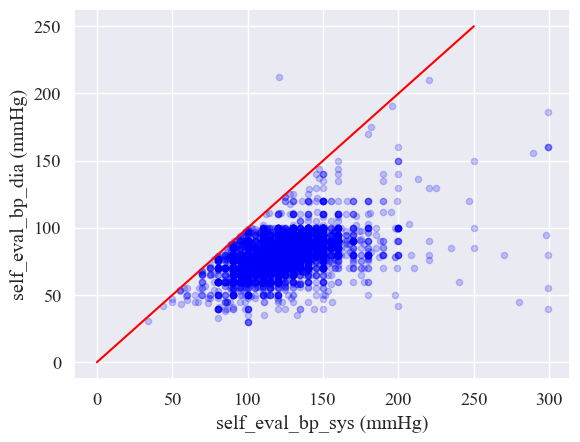
\includegraphics[width=\textwidth]{images/scatter-self-reported-bp.png}
        \caption{Self reported systolic and diastolic bp.}
        \label{fig:subplot1}
    \end{subfigure}
    \hfill
    \begin{subfigure}[b]{0.45\textwidth}
        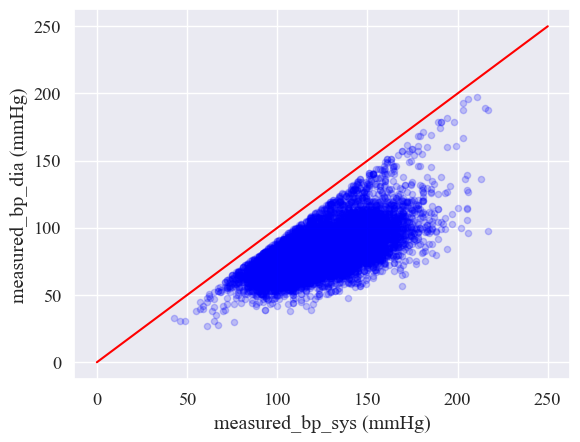
\includegraphics[width=\textwidth]{images/scatter-measured-bp.png}
        \caption{Measured systolic and diastolic bp.}
        \label{fig:subplot2}
    \end{subfigure}
    \vskip\baselineskip
    \begin{subfigure}[b]{0.45\textwidth}
        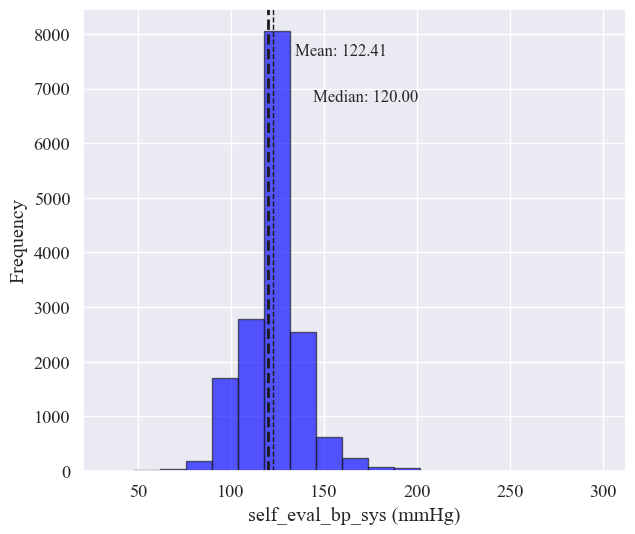
\includegraphics[width=\textwidth]{images/hist-self-reported-sys.png}
        \caption{Histogram of self reported systolic bp.}
        \label{fig:subplot3}
    \end{subfigure}
    \hfill
    \begin{subfigure}[b]{0.45\textwidth}
        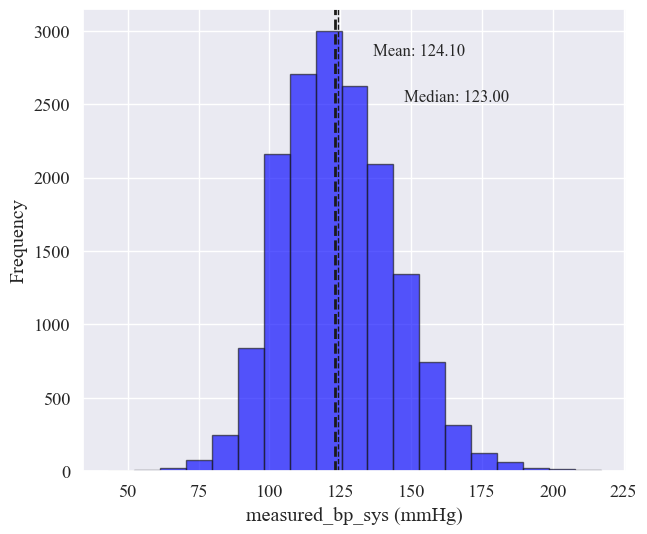
\includegraphics[width=\textwidth]{images/hist-measured-sys.png}
        \caption{Histogram of measured systolic bp.}
        \label{fig:subplot4}
    \end{subfigure}
    \caption{Histograms and scatter plots for the self reported and measured bp.}
    \label{fig:overall-bp}
\end{figure}

The scatter plot in Figure~\ref{fig:subplot1} compared to Figure~\ref{fig:subplot2} displays a substantial number of observations that 
deviate from the general trend, indicating the presence of a significant number of outliers.
To confirm this hypothesis, the histogram in Figure~\ref{fig:subplot3} 
shows a non-normal distribution, which suggests that the data may not conform to a Gaussian distribution. 
In contrast to the histogram in Figure~\ref{fig:subplot4} which approximates to a normal distribution.

These findings may indicate the presence of influential observations or underlying 
data generating processes that are not well captured by the model assumptions. 
Which may indicate that the self-reported blood pressure is not a reliable measure of the true blood pressure.
Hence, we decide to not further consider the variables \textit{Self-reported systolic} and \textit{Self-reported diastolic} blood pressures 
any longer in our analysis.

Figure~\ref{fig:boxplots-bp} (the following page) shows a series of boxplots for systolic and 
diastolic blood pressures w.r.t different variables. 
Figure~\ref{fig:subplot5} and Figure~\ref{fig:subplot6} show how the systolic and diastolic blood pressures vary
with the \textit{Federal state} variable. The main interest angle for this comparison 
is to see if the prevalence of hypertension (high blood pressure) can vary by geographic region, thus
leading to different blood pressure levels. Additionally, factors such as diet, lifestyle, and genetic predisposition 
could also contribute to regional differences in blood pressure. We observe that the overall median for diastolic blood pressure is
around 80 mmHg, which is considered normal. Similarly, the median for systolic blood pressure is around 125 mmHg, 
which is also in the norm. 
We discerne a homogeneous distribution of the blood pressure levels across the different federal states, 
except in the case of the Steiermark state, where there is a higher number of observations that are falling outside the interquarterile range
for both blood pressure levels. This might indicate that the prevalence of hypertension is higher in this region.

In Figure~\ref{fig:subplot7} and Figure~\ref{fig:subplot8} we want to see if there is enough evidence
to suggest that the blood pressure may vary seasonally. Recent studies have shown that blood pressure levels
tend to be higher in the winter and lower in the summer \citep{flint2019effect}.
Figure~\ref{fig:subplot7} indicates the presence of a seasonal pattern for the systolic blood pressure,
where the median is lower in the summer months (June, July, August) w.r.t October and November.
Even though we only have 26 observations in November.

Blood pressure can also vary depending on the day of the week. 
It tends to be higher on weekdays than on weekends. 
Seemingly, the stress of the work week can contribute to higher blood pressure levels \citep{juhanoja2016impact}.
Figure~\ref{fig:subplot8} tries to capture this effect. 
We observe that the median for systolic blood pressure is slightly higher on weekdays.
However, the difference is not significant enough to conclude that there is a difference in blood pressure levels.

\begin{figure}[H]
    \centering
    \begin{subfigure}[b]{0.45\textwidth}
        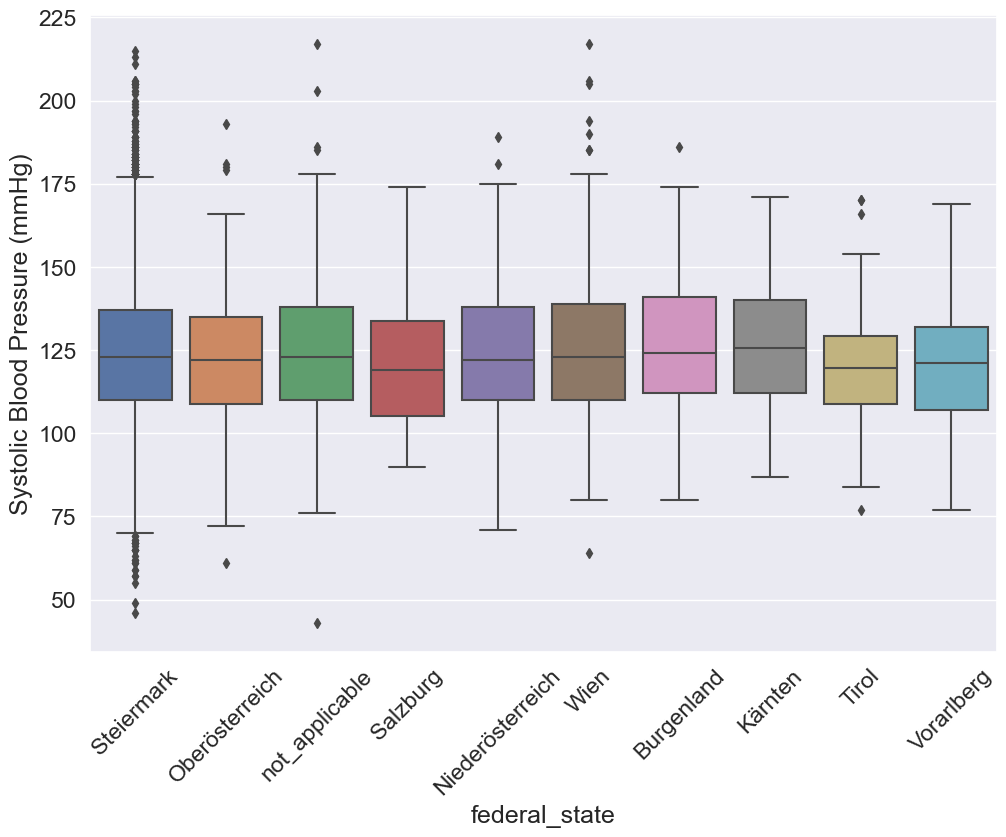
\includegraphics[width=\textwidth]{images/boxplot-state-sys.png}
        \caption{Systolic bp by federal state.}
        \label{fig:subplot5}
    \end{subfigure}
    \hfill
    \begin{subfigure}[b]{0.45\textwidth}
        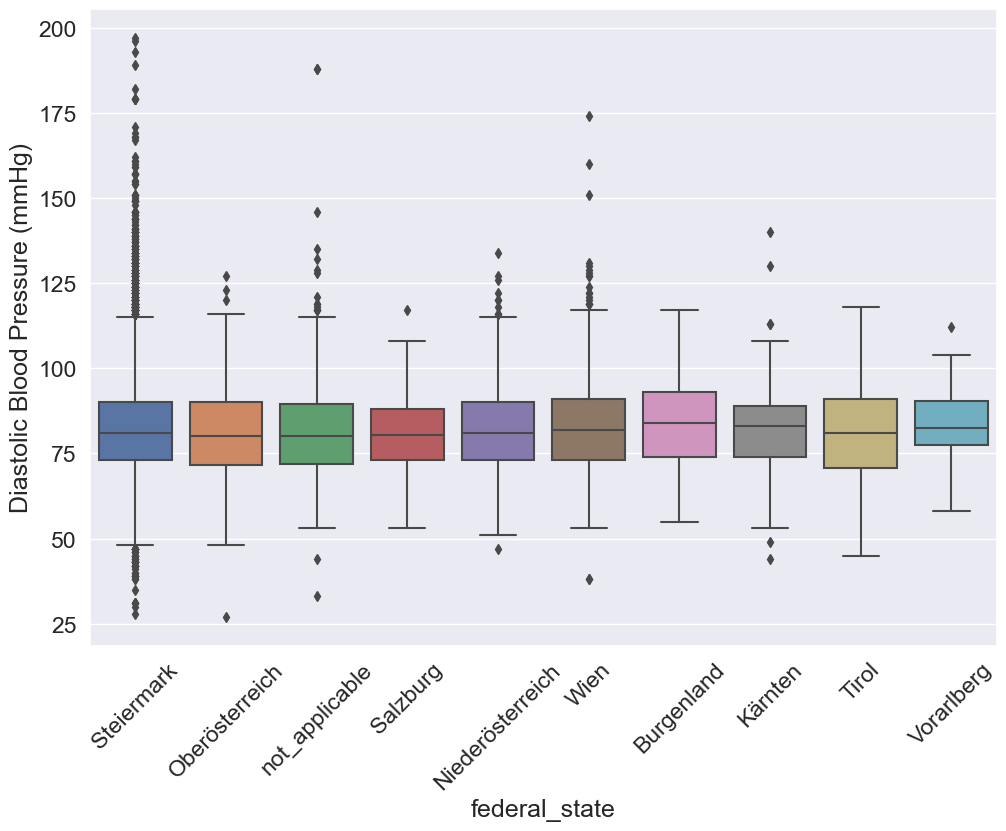
\includegraphics[width=\textwidth]{images/boxplot-state-dia.png}
        \caption{Diastolic bp by federal state.}
        \label{fig:subplot6}
    \end{subfigure}
    \vskip\baselineskip
    \begin{subfigure}[b]{0.45\textwidth}
        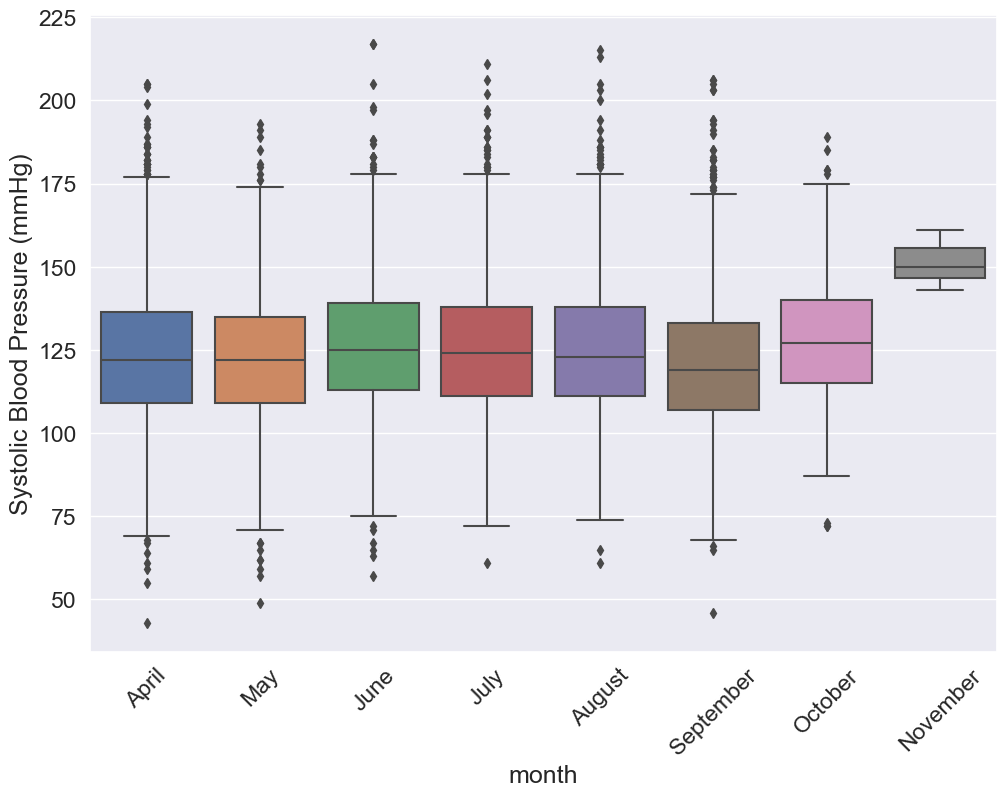
\includegraphics[width=\textwidth]{images/boxplot-month-sys.png}
        \caption{Systolic bp by month.}
        \label{fig:subplot7}
    \end{subfigure}
    \hfill
    \begin{subfigure}[b]{0.45\textwidth}
        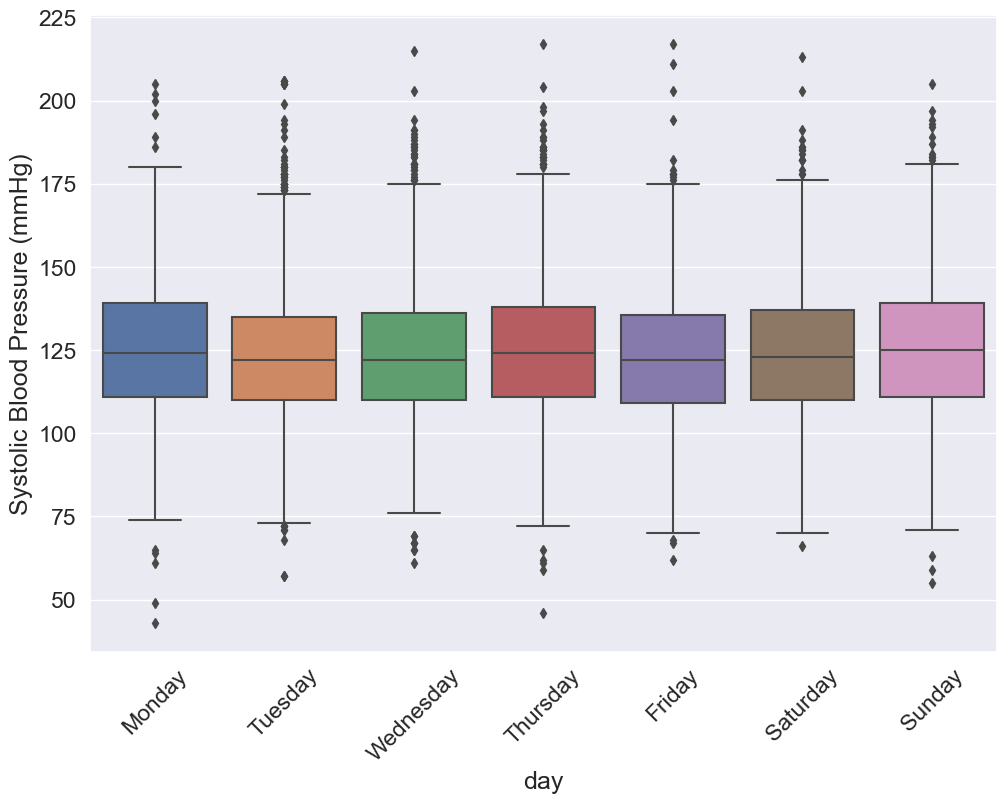
\includegraphics[width=\textwidth]{images/boxplot-day-sys.png}
        \caption{Systolic bp by day of the week.}
        \label{fig:subplot8}
    \end{subfigure}
    \caption{Boxplots for systolic and diastolic blood pressure w.r.t Autrian federal state, month, and day of the week.}
    \label{fig:boxplots-bp}
\end{figure}

Furthermore, we assessed how the systolic blood pressure varies with the \textit{Cholesterol level} and \textit{Smoking status} variables.
Figure~\ref{fig:subplot9} shows that the median for systolic blood pressure is higher for individuals with high cholesterol level.
This suggests that subjects with high cholesterol may have higher systolic blood pressure levels on average 
compared to those with normal cholesterol. 
This is consistent with previous research that has shown a positive association between high cholesterol and elevated blood 
pressure levels \citep{sakurai2011relationship}.

Conversely, Figure~\ref{fig:subplot10} shows that there is not enough evidence to conclude that
smoking status has an effect on systolic blood pressure levels (at least for the current sample size).

\begin{figure}[H]
    \centering
    \begin{subfigure}[b]{0.49\textwidth}
        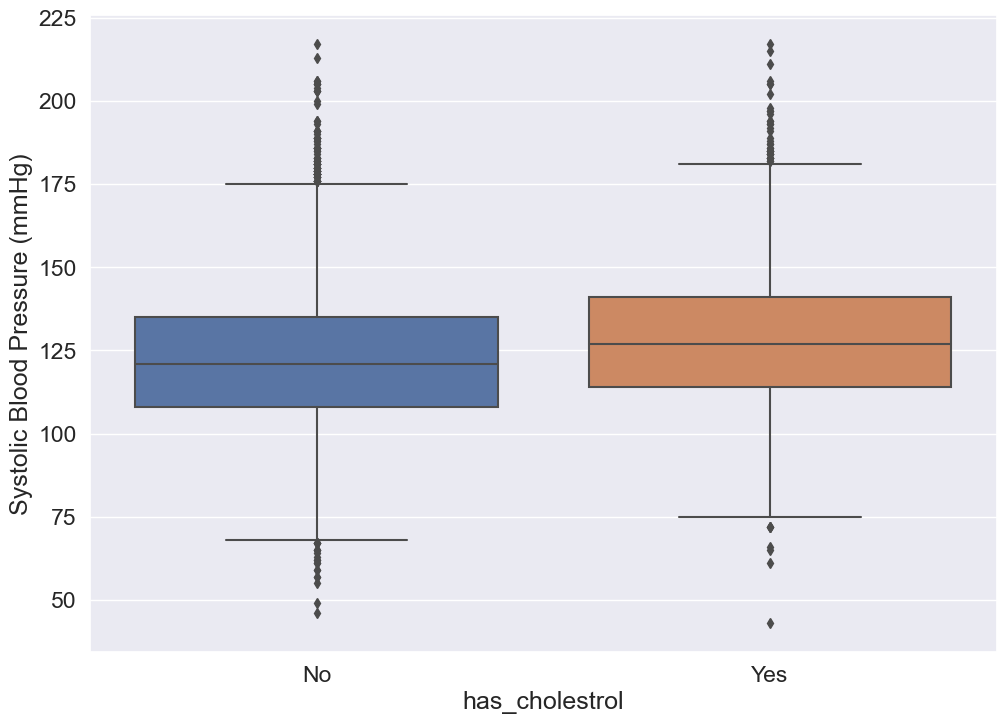
\includegraphics[width=\textwidth]{images/boxplot-cholesterol-sys.png}
        \caption{Systolic bp by cholesterol level.}
        \label{fig:subplot9}
    \end{subfigure}
    \hfill
    \begin{subfigure}[b]{0.49\textwidth}
        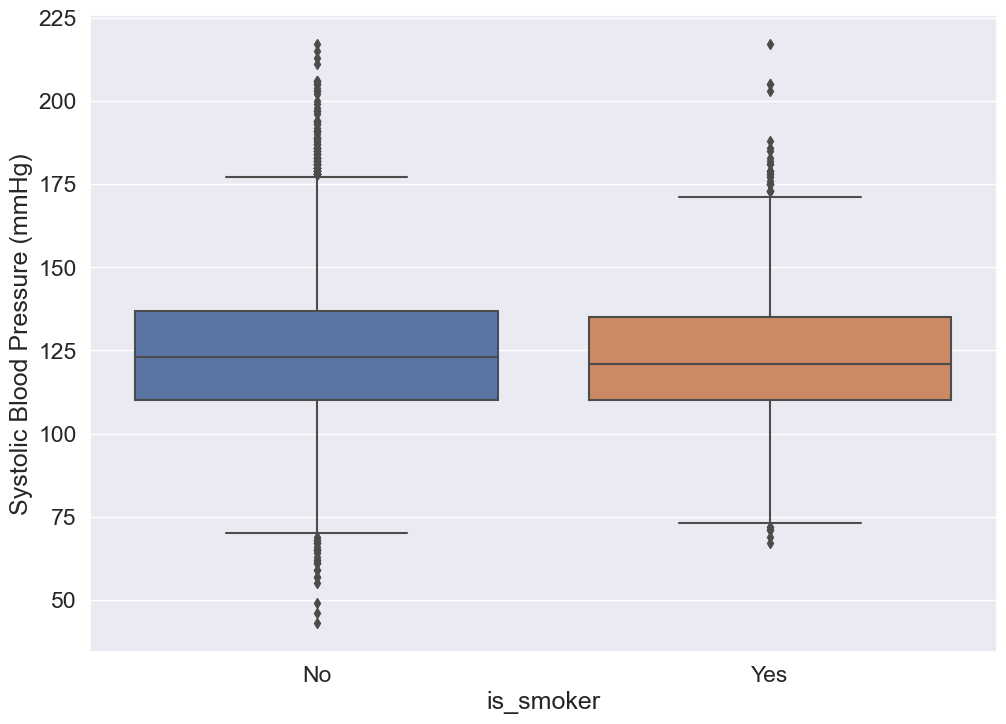
\includegraphics[width=\textwidth]{images/boxplot-smoker-sys.png}
        \caption{Systolic bp by smoking status.}
        \label{fig:subplot10}
    \end{subfigure}
    \caption{Boxplots for systolic blood pressure w.r.t cholesterol level and smoking status.}
\end{figure}


\subsection{Linear regression}
\label{subsec:Linear regrerssion analysis}

In this section, we fit two linear regression models to the data, taking the \textit{Measured Systolic blood pressure} 
and \textit{Measured Diastolic blood pressure} as the response variables.

We initially assess the normality assumption for the response variables using a QQ plot (c.f. section~\ref{subsec:qq-plot})
shown in Figure~\ref{fig:subplot11}. 


\begin{figure}[H]
    \centering
    \begin{subfigure}[b]{0.49\textwidth}
        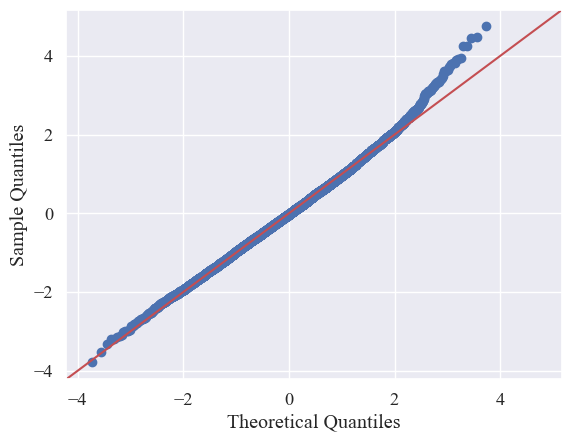
\includegraphics[width=\textwidth]{images/qq-plot-sys.png}
        \caption{Normal qq plot for the systolic bp.}
        \label{fig:subplot11}
    \end{subfigure}
    \hfill
    \begin{subfigure}[b]{0.49\textwidth}
        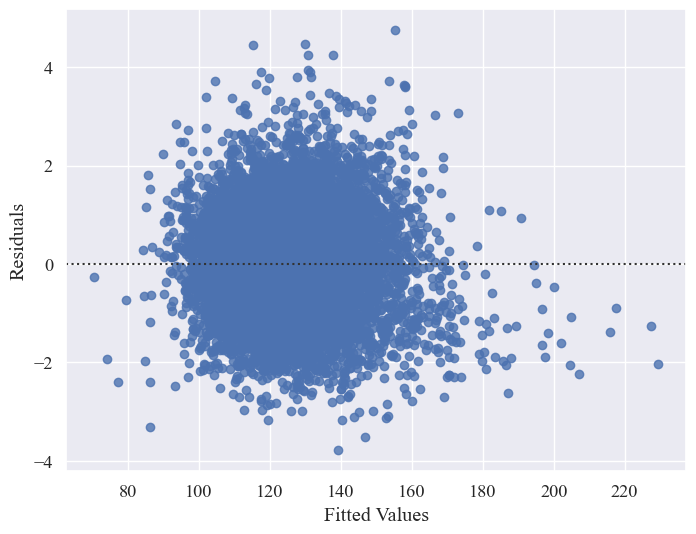
\includegraphics[width=\textwidth]{images/residual-plot-sys.png}
        \caption{Residual plot for the systolic bp.}
        \label{fig:subplot12}
    \end{subfigure}
    \caption{Normal qq plot (left) and residual plot (right) for the systolic blood pressure model.}
\end{figure}

We observe in Figure~\ref{fig:subplot11} that the data points align well with the theoretical quantiles, 
except for the upper tail. This suggests that the normality assumption is reasonable for the current sample size.

Figure~\ref{fig:subplot12} displays the residual plot (c.f. section~\ref{subsec:residual-plot}) for the systolic blood pressure model.
We observe that the residuals are evenly distributed around zero, which leads to conclude that the homoscedasticity assumption is 
also reasonable.

Conversely, we notice in Figure~\ref{fig:subplot13} that the data points do not align well with the theoretical quantiles.
This suggests that the normality assumption is somewhat alterated for the diastolic blood pressure model.
The residual plot in Figure~\ref{fig:subplot14}  
similarly indicates the presence of non-homoscedasticity. The residuals exhibit a fan shape, 
displaying unequal spread across the range of predicted values.
This means that the variability of the response variable differs across the levels of the predictor variables. 


\begin{figure}[H]
    \centering
    \begin{subfigure}[b]{0.49\textwidth}
        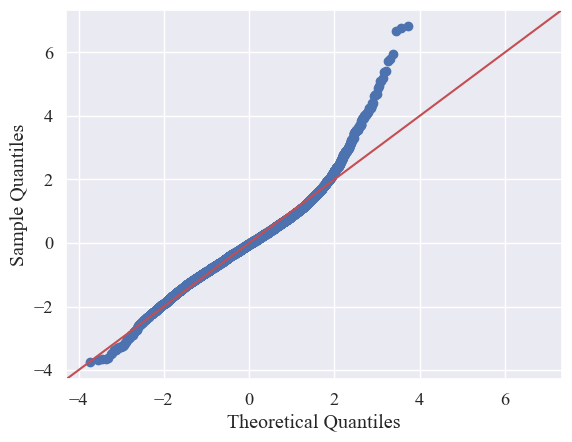
\includegraphics[width=\textwidth]{images/qqplot-dia.png}
        \caption{Normal qq plot for the systolic bp.}
        \label{fig:subplot13}
    \end{subfigure}
    \hfill
    \begin{subfigure}[b]{0.49\textwidth}
        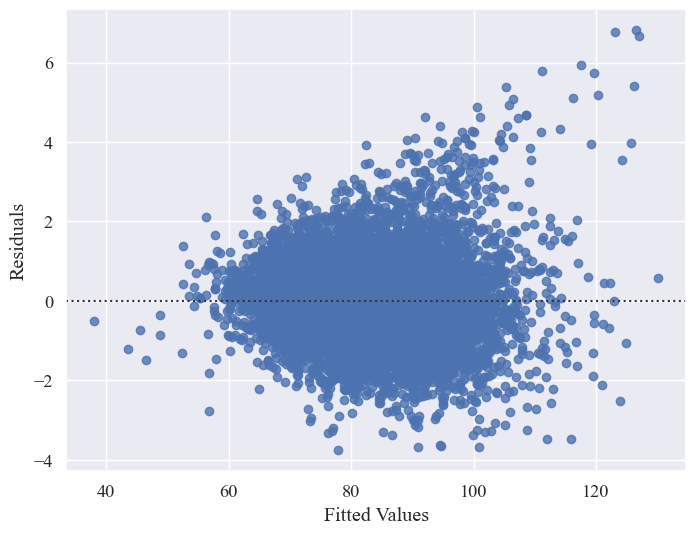
\includegraphics[width=\textwidth]{images/residual-plot-dia.png}
        \caption{Residual plot for the systolic bp.}
        \label{fig:subplot14}
    \end{subfigure}
    \caption{Normal qq plot (left) and residual plot (right) for the systolic blood pressure model.}
\end{figure}

Considering that the deviance from normality and homoscedasticity is not severe for both response variables, 
we proceed to fit a linear regression model to each blood pressure without transforming it.
The training set contains 10404 observations against 4460 observations for the testing set. 

We employ the linear regression model using the \textit{Diastolic blood pressure} as the response variable 
to demonstrate the interpretation of the coefficients. We only include the significant variables (c.f. section \ref{subsubsec:tests}).

Table~\ref{table:coefficients-dia} (c.f. Appendix) 
shows the results of the linear model fitted to the diastolic blood pressure.
The intercept coefficient of $18.7946$ indicates the estimated mean
diastolic blood pressure when all independent variables are equal to zero.
The rest of the coefficients are interpreted by an increase or decrease in the diastolic blood pressure
while holding the other features constant.

For the categorical variable \textit{Terminal},
terminal 2 has a positive coefficient of $1.94$, indicating that individuals 
in terminal 2 have a diastolic blood pressure that is, on average, $1.94$ mmHg higher than those in terminal 1 (reference level).
Similarly, terminal 3a has a negative coefficients of $-1.248$ indicating 
that measured individuals in terminal 3a have on average a lower diastolic blood pressure that those in terminal 1.

Felt health condition 2 has a negative coefficient of $-0.72$, showing 
that individuals who report feeling very good have a diastolic blood pressure that is, 
on average, $0.72$ mmHg lower than those who report feeling excellent.
Which shows that the diastolic blood pressure increases as the felt health condition decreases.
The gender has a positive relationship with the diastolic blood pressure and 
males have on average a higher diastolic blood pressure than females.

Individuals who report following a treatment have a lower diastolic blood pressure on average that those not in treatment.
The \textit{Systolic blood pressure} is also employed as a predictor for the diastolic blood pressure, and its coefficient is positive
indicating that higher measured systolic blood pressure is associated with higher diastolic blood pressure.
One unit increase in the systolic blood pressure is associated with a $0.61$ mmHg increase in the diastolic blood pressure.

The results of the model also indicate that the diastolic blood pressure 
decreases as the age increases. 
On average a one year older individual would lower his diastolic blood pressure by $0.09$ mmHg.
The hour of the day also plays a role,
the model suggests that on average the systolic blood pressure tends to be lower during later hours of the day. 

The weather conditions have also an impact on the diastolic blood pressure.
Specifically, higher temperature and higher humidity are associated with higher blood pressure.
One unit Celsius increment in the temperature is linked to $0.6$ mmHg increase in the diastolic blood pressure.

The linear model for the diastolic blood pressure has an $R^2$ value of $0.473$.
indicating that approximately 47.3\% of the variability in the response can be explained by the predictors. 
The adjusted $R^2$ value for the diastolic blood pressure model
is $0.471$. The linear model for the systolic blood pressure performs better with an $R^2$ value of $0.542$.
The \textit{Measured systolic blood pressure} is the most significant predictor in the model,
accounting for approximately $92\%$ of the total variability in the diastolic blood pressure.
Which explains why we decided to include it in the model despite the high correlation with the response variable.

\subsection{Ensemble Methods}
\label{subsec:Ensemble Methods}

\subsubsection*{Regression Tree and Random Forest}
\label{subsec:Regression Trees}

The set of hyperparameters (c.f. section~\ref{subsec:Regression Trees}) choosen for the regression tree and the random forest model for
the systolic blood pressure are the following:

\begin{itemize}
    \item Max depth: 10.
    \item Max number of features: 40.
    \item Minimum sample of leaves per node: 70.
    \item Splitter: Best algorithm.
\end{itemize} 

We use the same training/testing split as in the linear regression model.
We present the results of the regression tree models on the diastolic blood pressure in Table~\ref{table:base-models-sys}.

\begin{table}[H]
    \centering
    \scalebox{1.0}{
        \begin{tabular}{|l||r|r|r|r|r|r|}
            \hline
            Model & Train Mean Sq Error & Test Mean Sq Error & Train R2 & Test R2 \\ \hline
            Regression Tree (Base) & 0.490 & 217.600 & 1.000 & -0.100 \\ 
            Random Forest (Base) & 15.950 & 114.530 & 0.920 & 0.420 \\
            \hline
        \end{tabular}
    }
    \caption{Results of the base regression tree and random forest models for the systolic blood pressure.}
    \label{table:base-models-sys} 
\end{table}

From Table~\ref{table:base-models-sys} we conclude the following resutls:
The average squared difference between the predicted and actual diastolic blood pressure values on the training data is 0.49. 
This indicates a relatively low level of error in the model's predictions for the training dataset.
In comparison the mean squred error on the training dataset for the random forest model is 15.95.
Which indicates that the random forest model exhibits a higher level of error in its predictions for the training dataset.

For the test set, the mean squared error for the Random forest is lower than the regression tree model.
Which shows that the random forest model performs better than the regression tree model for the test dataset,
and therefore, the random forest model is less prone to overfitting and generalizes better.

The $R^2$ for both models in the training set is very high indicating a high level of overfitting.
Nontheless, the random forest model outperforms the regression tree model in the test set, 
explaining 42\% of the variability in the diastolic blood pressure. 
This number is similar to the previous linear regression model.


\subsection{Evaluation of the goodness of fit}
\label{subsec:Evaluation of the goodness of fit}

\subsubsection*{Best subset of explanatory variables}
\label{subsubsec:Best subset of explanatory variables}

Using the best subset selection algorithm explained in section~\ref{subsec:Best Subset Selection}, we iteratively fit multiple
linear models to the data and select the best set based on the MSE criterion.

Table \ref{tab:best-subset} shows the results of the best subset selection algorithm for the diastolic blood pressure.
We observe that the best subset selection algorithm does not improve the performance of the base linear model, 
the adjusted $R^2$ is approximately the same for both models.

\begin{table}[H]
    \centering
    \scalebox{0.85}{
    \begin{tabular}{|l||l|r|r|r|r|}
        \hline
     Model & Train Mean Sq Error & Test Mean Sq Error & Train Adjusted R2 & Test Adjusted R2 \\ \hline
    LM (Base) & 109.906 & 108.071 & 0.455 & 0.451 \\ \hline
    LM (Best Subset) & 108.053 & 110.150 & 0.453 & 0.454 \\ \hline
    \end{tabular}%
    }
    \caption{Results of the best subset selection algorithm for the diastolic blood pressure.}
    \label{tab:best-subset}
    \end{table}

\subsubsection*{Fine tuning with cross-validation}

For the regression tree models we performed an additional step to improve on the base model.
We used the cross-validation (explained in section~\ref{subsec:Fine Tuning using Cross-Validation}) method to fine tune the hyperparameters of the regression tree model
and the random forest model.

Table \ref{tab:cv} shows the results of the fine tunned regression tree and random forest models for the diastolic blood pressure.
For both models the fine tuning step improves the performance of the base model on the test set.
Leading to an Adjusted $R^2$ of $0.460$ for the regression tree model and $0.470$ for the random forest model.

\begin{table}[H]
    \centering
    \scalebox{0.85}{
    \begin{tabular}{|l||l|r|r|r|r|}
        \hline
     Model & Train Mean Sq Error & Test Mean Sq Error & Train Adjusted R2 & Test Adjusted R2 \\ \hline
    Reg Tree (Base) & 0.490 & 217.600 & 1.000 & -0.110 \\ \hline
    Reg Tree (Fine tunned) & 100.350 & 105.500 & 0.500 & 0.460 \\ \hline
    R Forest (Base) & 15.950 & 114.530 & 0.920 & 0.420 \\ \hline
    R Forest (Fine tunned) & 97.310 & 103.100 & 0.520 & 0.470 \\ \hline
    \end{tabular}%
    }
    \caption{Results for the fine tunned regression tree and random forest models for the diastolic blood pressure.}
    \label{tab:cv}
    \end{table}


To draw a comparison between the linear regression and the regression tree models
we can observe that 
both models exhibit similar performance in terms of explaining the variability in the response variable. 
The adjusted $R^2$ values for both models are very close, suggesting that they capture a similar 
proportion of the total variation in the data.

The linear model offers straightforward interpretability as it provides the coefficients that represent the relationship between the predictors and the response variable. 
Conversely, the interpretation of a regression tree is more intuitive (no parameters to interpret) as it involves hierarchical splits based on predictor values.

The ARIMA model is a time series model that is used to predict future values based on past values.
The mathematical formulation of the model is as follows:

\begin{equation}
    \label{eq:arima}
    y_t = c + \phi_1 y_{t-1} + \phi_2 y_{t-2} + \dots + \phi_p y_{t-p} + \epsilon_t + \theta_1 \epsilon_{t-1} + \theta_2 \epsilon_{t-2} + \dots + \theta_q \epsilon_{t-q}   
\end{equation}

\section{Summary}
\label{sec:Summary}

In this case study we focused on a dataset that contains information about 
blood pressure measurements taken from visitors to the \textit{Wege zur Gesundheit} 
exhibition held in the city of Bruck an der Mur in 2006.
The event aimed to promote healthy living and featured various health-related activities.

The dataset comprises 16,386 measurements of systolic and diastolic blood pressure, 
as well as 18 other parameters that describe the geographic and physiological characteristics 
of the visitors. The aim is to model the systolic and diastolic blood pressure based on the
other parameters.

We initially started by a pre-processing phase, 
where we performed feature engineering on some of the categorical variables in our dataset.
Initially, we created a new variable called \textit{Age} by calculating the difference 
between the date of birth and the date of blood pressure measurements.
We also extracted the variables \textit{Year}, \textit{Month} and \textit{Day} from the date of blood pressure measurements.
Furthermore, we split the \textit{Terminal} 3 variable into two subgroups, "3a" and "3b," after the measurement device was changed.
Additionally, we incorporated meteorological data, such as temperature, humidity, and weather conditions, 
in our analysis. Specifically, we incorporated the meteorological readings taken on the day of the blood pressure measurements.
Lastly, we removed all inconsistent observations from the dataset, and dummy encoded the categorical variables,
amounting to a total of 26 usable features for our analysis.


We thereafter, proceeded to explore the data applying descriptive analysis methods to grasp indepth insight into it.
We studied the distribution of the systolic and diastolic blood pressures in their two forms: 
measured and self-reported. We concluded that
the distribution of the self-reported blood pressure suggests the possibility of influential observations or data generating processes 
not well captured by the model assumptions.
Thus, indicating that the measurements may not be reliable. We therefore, decided to focus our analysis on the measured blood pressure.

We also examined the potential correlation between blood pressure and various factors, 
such as federal state, in order to determine if there was a variation in hypertension prevalence across different geographic regions.
The analysis revealed generally uniform distribution of blood pressure levels across all states.
We also investigated the relationship between blood pressure and seasonality, and found evidence to suggest that blood pressure levels may vary seasonally.
We further explored possible correlations between health-related factors and blood pressure levels.
We found that there is a positive association between high cholesterol and elevated blood pressure levels.   

In the course of the analysis, 
we assessed if the normality assumptions of the linear model were met by the response variables:
\textit{Measured Diastolic blood pressure} and \textit{Measured Systolic blood pressure}.
And then proceeded to fit two linear models for each target blood pressure.
Both linear models perfomed in a moderately effective way,
with the Systolic model performing slightly better than the Diastolic model, averaging an $R^2$ value of 0.57 against
0.47 for the diastolic model. 
We also found out that for the diastolic model, $92\%$ of the variance is explained by the systolic blood pressure as a predictor.
This is not surprising as the systolic blood pressure is a strong predictor of the diastolic blood pressure.

Alongside the linear models, we also fitted a regression tree and random forest model for each target blood pressure.
We also used fine-tuning algortihms witht the MSE as a criterion to improve on the current state of our models.
We used best subset selection to select the best predictors for the linear models, and
used cross-validation to fine-tune the regression tree and random forest models.
The results showed minimal differences, with only marginal improvements observed. 
The random forest model performed slightly better than all other models with an adjusted $R^2$ 
on the testing set of $0.47$ for the diastolic blood pressure and $0.54$ for the systolic blood pressure. 

Finally, the significant model's parameters were interpreted and the results were discussed.

In this case study we assumed that the relationship between the response variable and the regressors is linear.
Even though, in most realistic cases the linear model is no longer relevant and for further studies it would be interesting
to explore advanced regression models like the Robust regression or even the Generalized Additive Models (GAMs) that can capture non-linear relationships.


\newpage
\addcontentsline{toc}{section}{Bibliography}
\renewcommand\refname{Bibliography} 
\bibliographystyle{plainnat}
\bibliography{references}

\appendix 
\addsec{Appendix}

\subsection*{Additional Tables}

Table \ref{table:coefficients-dia} (following page) shows the list of regressors and their coefficients for the linear model fitted to the diastolic blood pressure.

\begin{table}[htb]
    \begin{center}
        \captionabove{Summary of the Linear regression model fitted to the Diastolic blood pressure.}
        \begin{tabular}{|l||c|c|c|c|cc|}
            \hline
        \textbf{Variable name}                    & \textbf{coef} & \textbf{std err} & \textbf{t} & \textbf{P$> |$t$|$} & \textbf{[0.025} & \textbf{0.975]}  \\ \hline
        
        \textbf{Intercept}                        &      18.7946  &        2.392     &     7.856  &         0.000        &       14.105    &       23.484     \\ \hline
        \textbf{terminal\_2}                      &       1.9449  &        0.247     &     7.876  &         0.000        &        1.461    &        2.429     \\
        \textbf{terminal\_3a}                     &      -1.2479  &        0.419     &    -2.981  &         0.003        &       -2.068    &       -0.427     \\
        \textbf{terminal\_3b}                     &      -0.6710  &        0.290     &    -2.316  &         0.021        &       -1.239    &       -0.103     \\ \hline
        \textbf{federal\_state\_Kärnten}          &      -2.2591  &        1.471     &    -1.536  &         0.125        &       -5.143    &        0.625     \\
        \textbf{federal\_state\_Niederösterreich} &      -1.6394  &        1.302     &    -1.259  &         0.208        &       -4.192    &        0.913     \\
        \textbf{federal\_state\_Oberösterreich}   &      -1.7391  &        1.444     &    -1.204  &         0.229        &       -4.571    &        1.092     \\
        \textbf{federal\_state\_Salzburg}         &      -0.4074  &        1.777     &    -0.229  &         0.819        &       -3.890    &        3.075     \\
        \textbf{federal\_state\_Steiermark}       &      -1.4835  &        1.160     &    -1.279  &         0.201        &       -3.757    &        0.789     \\
        \textbf{federal\_state\_Tirol}            &      -1.6314  &        1.891     &    -0.863  &         0.388        &       -5.337    &        2.074     \\
        \textbf{federal\_state\_Vorarlberg}       &       0.5143  &        2.923     &     0.176  &         0.860        &       -5.215    &        6.243     \\
        \textbf{federal\_state\_Wien}             &      -0.9295  &        1.292     &    -0.720  &         0.472        &       -3.462    &        1.603     \\
        \textbf{federal\_state\_not\_applicable}  &      -1.8763  &        1.394     &    -1.346  &         0.178        &       -4.609    &        0.856     \\ \hline
        \textbf{felt\_health\_condition\_2}       &      -0.7195  &        0.229     &    -3.140  &         0.002        &       -1.169    &       -0.270     \\
        \textbf{felt\_health\_condition\_3}       &      -0.2442  &        0.327     &    -0.746  &         0.456        &       -0.886    &        0.398     \\
        \textbf{felt\_health\_condition\_4}       &      -0.3979  &        0.969     &    -0.411  &         0.681        &       -2.296    &        1.501     \\
        \textbf{felt\_health\_condition\_5}       &       3.7336  &        1.613     &     2.314  &         0.021        &        0.571    &        6.896     \\ \hline
        \textbf{gender\_m}                        &       1.2023  &        0.208     &     5.779  &         0.000        &        0.795    &        1.610     \\ \hline
        \textbf{is\_smoker\_True}                 &       0.0357  &        0.282     &     0.126  &         0.899        &       -0.518    &        0.589     \\ \hline
        \textbf{is\_diabetic\_True}               &      -0.2325  &        0.291     &    -0.800  &         0.424        &       -0.802    &        0.337     \\ \hline
        \textbf{has\_cholestrol\_True}            &       0.1427  &        0.270     &     0.529  &         0.597        &       -0.386    &        0.671     \\ \hline
        \textbf{in\_treatment\_True}              &      -1.6391  &        0.329     &    -4.985  &         0.000        &       -2.284    &       -0.995     \\ \hline
        \textbf{month\_Aug}                       &       0.7421  &        0.786     &     0.944  &         0.345        &       -0.799    &        2.283     \\
        \textbf{month\_Jul}                       &      -0.5602  &        0.898     &    -0.624  &         0.533        &       -2.321    &        1.200     \\
        \textbf{month\_Jun}                       &       0.4529  &        0.825     &     0.549  &         0.583        &       -1.165    &        2.071     \\
        \textbf{month\_May}                       &       0.5684  &        0.778     &     0.731  &         0.465        &       -0.956    &        2.092     \\
        \textbf{month\_Nov}                       &      21.4579  &       10.456     &     2.052  &         0.040        &        0.962    &       41.954     \\
        \textbf{month\_Oct}                       &      -3.2398  &        0.782     &    -4.142  &         0.000        &       -4.773    &       -1.707     \\
        \textbf{month\_Sep}                       &      -2.7086  &        0.791     &    -3.425  &         0.001        &       -4.259    &       -1.158     \\ \hline
        \textbf{day\_Monday}                      &       0.1772  &        0.426     &     0.416  &         0.677        &       -0.658    &        1.012     \\
        \textbf{day\_Saturday}                    &       0.4438  &        0.383     &     1.157  &         0.247        &       -0.308    &        1.195     \\
        \textbf{day\_Sunday}                      &       0.2094  &        0.362     &     0.578  &         0.563        &       -0.500    &        0.919     \\
        \textbf{day\_Thursday}                    &      -0.9265  &        0.401     &    -2.312  &         0.021        &       -1.712    &       -0.141     \\
        \textbf{day\_Tuesday}                     &      -1.1554  &        0.435     &    -2.659  &         0.008        &       -2.007    &       -0.304     \\
        \textbf{day\_Wednesday}                   &      -1.0129  &        0.418     &    -2.421  &         0.015        &       -1.833    &       -0.193     \\ \hline
        \textbf{measured\_bp\_sys}                &       0.5290  &        0.006     &    90.745  &         0.000        &        0.518    &        0.540     \\ \hline
        \textbf{age}                              &      -0.0892  &        0.007     &   -12.168  &         0.000        &       -0.104    &       -0.075     \\ \hline
        \textbf{hour}                             &      -0.0898  &        0.046     &    -1.952  &         0.051        &       -0.180    &        0.000     \\ \hline
        \textbf{temp}                             &       0.6937  &        0.155     &     4.466  &         0.000        &        0.389    &        0.998     \\ \hline
        \textbf{humidity}                         &       0.0669  &        0.016     &     4.136  &         0.000        &        0.035    &        0.099     \\ \hline
        \textbf{temp\_min}                        &      -0.3059  &        0.101     &    -3.031  &         0.002        &       -0.504    &       -0.108     \\ \hline
        \textbf{temp\_max}                        &      -0.3587  &        0.077     &    -4.634  &         0.000        &       -0.510    &       -0.207     \\ \hline
        \hline
        
        \end{tabular}
        \label{table:coefficients-dia}
        \end{center}
    \end{table}

\end{document}